    
\documentclass{article}
\usepackage[utf8]{inputenc}
\usepackage[spanish]{babel}
\usepackage{listings}
\usepackage{subfigure}
\usepackage{graphicx}
\usepackage{url}
\usepackage{multirow}
\usepackage{color}
\usepackage{booktabs}

\usepackage[margin=3cm,twoside]{geometry} 
\setlength{\parindent}{0pt}
\setlength{\parskip}{1em}


\definecolor{mygreen}{rgb}{0,0.6,0}
\definecolor{mygray}{rgb}{0.5,0.5,0.5}
\definecolor{mymauve}{rgb}{0.58,0,0.82}
\lstset{ 
  backgroundcolor=\color{white},   % choose the background color; you must add \usepackage{color} or \usepackage{xcolor}; should come as last argument
  basicstyle=\footnotesize,        % the size of the fonts that are used for the code
  breakatwhitespace=false,         % sets if automatic breaks should only happen at whitespace
  breaklines=true,                 % sets automatic line breaking
  captionpos=b,                    % sets the caption-position to bottom
  commentstyle=\color{mygreen},    % comment style
  deletekeywords={...},            % if you want to delete keywords from the given language
  escapeinside={\%}{)},          % if you want to add LaTeX within your code
  extendedchars=true,              % lets you use non-ASCII characters; for 8-bits encodings only, does not work with UTF-8
  firstnumber=1,                % start line enumeration with line 1000
  frame=single,	                   % adds a frame around the code
  keepspaces=true,                 % keeps spaces in text, useful for keeping indentation of code (possibly needs columns=flexible)
  keywordstyle=\color{blue},       % keyword style
  language=Octave,                 % the language of the code
  morekeywords={*,...},            % if you want to add more keywords to the set
  numbers=left,                    % where to put the line-numbers; possible values are (none, left, right)
  numbersep=5pt,                   % how far the line-numbers are from the code
  numberstyle=\tiny\color{mygray}, % the style that is used for the line-numbers
  rulecolor=\color{black},         % if not set, the frame-color may be changed on line-breaks within not-black text (e.g. comments (green here))
  showspaces=false,                % show spaces everywhere adding particular underscores; it overrides 'showstringspaces'
  showstringspaces=false,          % underline spaces within strings only
  showtabs=false,                  % show tabs within strings adding particular underscores
  stepnumber=1,                    % the step between two line-numbers. If it's 1, each line will be numbered
  stringstyle=\color{mymauve},     % string literal style
  tabsize=2,	                   % sets default tabsize to 2 spaces
  title=\lstname                  % show the filename of files included with \lstinputlisting; also try caption instead of title
}


\begin{document}

\title{Tarea No.4: Rectificada}
\author{Dayli Machado (5275)}
\date{\today}
\maketitle

\section{Objetivo}

Determinar mediante un diseño de experimentos empleando el análisis de varianzas de un factor y otras pruebas estadísticas la influencia que puede tener en la variable dependiente\textit{ tiempo de ejecución}, el  orden y la densidad del grafo así como el generador de grafos y el algoritmo de flujo máximo seleccionado.

\section{Generador de grafos, algoritmos de flujo máximo empleados y generación del .csv }

De los tipos de generador de grafos se seleccionaron los generadores aleatorios y dentro de estos el grupo de tres modelos de generadores de grafos desarrollados por \textit{Watts y Strogatz} \cite{generadoraws}. Estos permiten de una forma relativamente sencilla y con menor número de parámetros generar los grafos. Una propiedad importante de estos tres generadores de grafos es que se desarrollan bajo la teoría de red de mundos pequeños, bajo esta teoría se crean nodos principales los cuales están alejados entre sí y generalmente se grafican más grandes que los demás, alrededor de estos se crean nodos que sí son vecinos entre sí y se grafican con tamaños más pequeños, de esta manera se garantiza la propiedad de crear grupos dentro del mismo grafo permitiendo que sea relativamente fácil realizar la visita entre todos los nodos. Esta propiedad refleja mejor el comportamiento de fenómenos reales como las redes eléctricas, neuronales y sociales. Otra propiedad de estos generadores de grafos es que la distancia esperada entre dos nodos elegidos al azar crece de manera proporcional al logaritmo de la cantidad de nodos de la red mientras no se trate de los nodos que están más agrupados, propiedad que detectaron los creadores a partir del comportamiento real de diferentes fenómenos \cite{wys}. De ahí que los generadores de grafos seleccionados fueron los siguientes:

\begin{itemize}
\item \textit{grafo de Watts Strogatz Newman }
\item \textit{grafo de Watts Strogatz }
\item \textit{grafo de Watts Strogatz Conectado}
\end{itemize}
%%\newpage
%\lstinputlisting[language=Python, firstline=9, lastline=58]{codigomadre.py}

Los algoritmos de flujo máximo seleccionados fueron los siguientes:
\begin{itemize}
\item \textit{Algoritmo Boykov-Kolmogorov }
\item \textit{Algoritmo de flujo máximo}
\item \textit{Algoritmo Edmonds-Karp}
\end{itemize} 


El algoritmo de máximo flujo determina la ruta a través de la cual puede pasar el máximo flujo, de ahí que uno de los parámetros que requiere es la capacidad, y un su defecto la asume como infinita \cite{mf}. Se recomienda emplearlo en grafos dirigidos pero funciona también para no dirigidos.

El algoritmo de \textit{Boykov-Kolmogorov} encuentra el flujo máximo de un sólo producto este devuelve la red residual resultante después de calcular el flujo máximo, debe tener capacidad en sus pesos sino los toma como infinitos \cite{bk}. Se recomienda para grafos dirigidos, aunque puede emplearse también para no dirigidos. 

El algoritmo de \textit{Edmonds-Karp} calcula el flujo máximo de un producto y además devuelve la red residual del mismo, se emplea en grafos dirigidos y no dirigidos. Al igual que los anteriores debe asignarse una capacidad sino la toma como infinita \cite{ek}.

A continuación se muestra el fragmento de código desarrollado para generar los grafos empleando los diferentes algoritmos:

\newpage
\lstinputlisting[language=Python, firstline=12, lastline=18]{Tarea4csvfinal.py}
\lstinputlisting[language=Python, firstline=33, lastline=34]{Tarea4csvfinal.py}

En el siguiente fragmento se muestra como se ha desarrollado el código para asignar el peso normalmente distribuido a cada arista, apoyándose en \cite{tutorialpython}.

\lstinputlisting[language=Python, firstline=50, lastline=72]{Tarea4csvfinal.py}

Después se genera el .csv con la siguiente estructura:
\newpage
\lstinputlisting[language=Python, firstline=80, lastline=91]{Tarea4csvfinal.py}

Con los datos generados se pasa a realizar el análisis estadístico de los mismos.


\section{Análisis de varianza (ANOVA), prueba de \textit{Tukey} y relación general entre factores} 

Para realizar el análisis del comportamiento de la variable dependiente \textit{tiempo de ejecución} con respecto a cada factor a analizar se realizó un análisis de varianza (ANOVA) para cada factor.

En el caso del análisis de la densidad vs \textit{tiempo de ejecución} se convirtieron los valores de densidad  a rangos de valores genéricos, para ello se realizó un histograma para dividir los rangos y llevarlos a una escala cualitativa en correspondencia con el arreglo obtenido del \textit{bins}. El arreglo se muestra en el cuadro siguiente y el histograma en la figura \ref{fig:Fig1} de la página \pageref{fig:Fig1}

\begin{figure}[htbp]
    \centering
    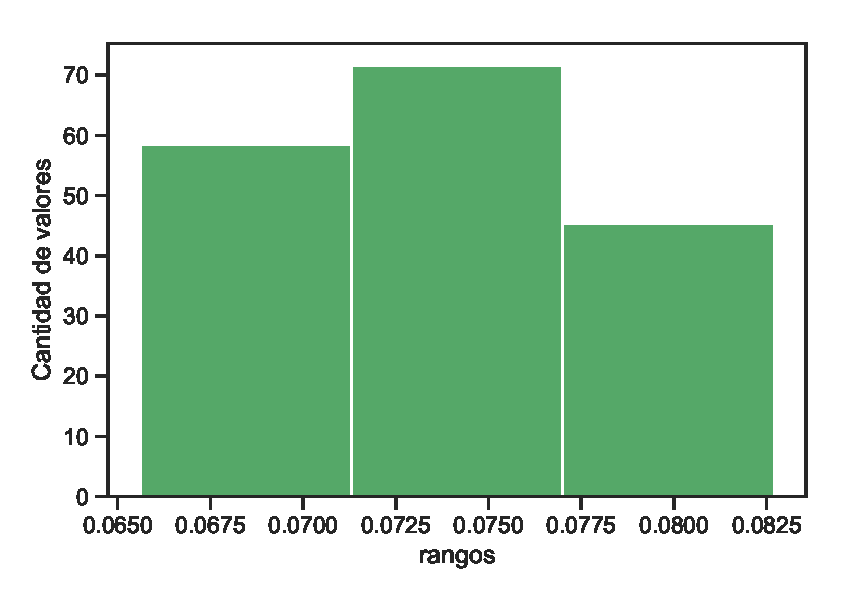
\includegraphics[scale=0.6]{Imagenes/Histogramadensidad.eps}
    \caption{Histograma para determinar escala de densidad}
    \label{fig:Fig1}
\end{figure}

Visualmente del histograma es complejo identificar los rangos correctos para establecer la escala, por lo que se trabajó con el arreglo de rangos que devuelve el histograma siguiente:

% Table generated by Excel2LaTeX from sheet 'Arreglodensid'
\begin{table}[htbp]
  \centering
  \caption{Arreglo para los rangos de densidad}
    \begin{tabular}{cccc}
    \toprule
    0.0656 & 0.0713 & 0.077 & 0.0827 \\
    \bottomrule
    \end{tabular}%
  \label{tab:addlabel}%
\end{table}%

A continuación se muestran los cuadros que resumen el resultado del ANOVA para cada factor:

% Table generated by Excel2LaTeX from sheet 'Tabla_ANOVAalgoritmo_flujo'
\begin{table}[htbp]
  \centering
  \caption{ANOVA del tiempo de ejecución vs algoritmo de flujo}
    \begin{tabular}{lrrrlll}
    \toprule
    \textbf{Source} & \multicolumn{1}{l}{\textbf{SS}} & \multicolumn{1}{l}{\textbf{DF}} & \multicolumn{1}{l}{\textbf{MS}} & \textbf{F} & \textbf{p-unc} & \textbf{np2} \\
    \midrule
    algoritmo\_flujo & 1.76  & 2     & 0.88  & \multicolumn{1}{r}{3.46} & \multicolumn{1}{r}{0.03} & \multicolumn{1}{r}{0.00} \\
    Within & 455.99 & 1797  & 0.25 &      &   & \\
    \bottomrule
    \end{tabular}%
  \label{tab:addlabel}%
\end{table}%

% Table generated by Excel2LaTeX from sheet 'Tabla_ANOVAconvlogdensidad'
\begin{table}[htbp]
  \centering
  \caption{ANOVA del tiempo de ejecución vs densidad del grafo}
    \begin{tabular}{lrrrlll}
    \toprule
    \textbf{Source} & \multicolumn{1}{l}{\textbf{SS}} & \multicolumn{1}{l}{\textbf{DF}} & \multicolumn{1}{l}{\textbf{MS}} & \textbf{F} & \textbf{p-unc} & \textbf{np2} \\
    \midrule
    convlogdensidad & 61.56 & 2     & 30.78 & \multicolumn{1}{r}{139.62} & \multicolumn{1}{r}{0.00} & \multicolumn{1}{r}{0.13} \\
    Within & 396.19 & 1797  & 0.22  &     &      &  \\
    \bottomrule
    \end{tabular}%
  \label{tab:addlabel}%
\end{table}%

% Table generated by Excel2LaTeX from sheet 'Tabla_ANOVAgenerador'
\begin{table}[htbp]
  \centering
  \caption{ANOVA del tiempo de ejecución vs generador}
    \begin{tabular}{lrrrlll}
    \toprule
    \textbf{Source} & \multicolumn{1}{l}{\textbf{SS}} & \multicolumn{1}{l}{\textbf{DF}} & \multicolumn{1}{l}{\textbf{MS}} & \textbf{F} & \textbf{p-unc} & \textbf{np2} \\
    \midrule
    generador & 3.09& 2     & 1.54& \multicolumn{1}{r}{6.11} & \multicolumn{1}{r}{0.00} & \multicolumn{1}{r}{0.00} \\
    Within & 454.66 & 1797  & 0.253 &     &      &  \\
    \bottomrule
    \end{tabular}%
  \label{tab:addlabel}%
\end{table}%


% Table generated by Excel2LaTeX from sheet 'Tabla_ANOVAvertices'
\begin{table}[htbp]
  \centering
  \caption{ANOVA del tiempo de ejecución vs vértices}
    \begin{tabular}{lrrrlll}
    \toprule
    \textbf{Source} & \multicolumn{1}{l}{\textbf{SS}} & \multicolumn{1}{l}{\textbf{DF}} & \multicolumn{1}{l}{\textbf{MS}} & \textbf{F} & \textbf{p-unc} & \textbf{np2} \\
    \midrule
    vertices & 433.22 & 3     & 144.40 & \multicolumn{1}{r}{10571.46} & \multicolumn{1}{r}{0} & \multicolumn{1}{r}{0.94} \\
    Within & 24.53 & 1796  & 0.014 &     &      &  \\
    \bottomrule
    \end{tabular}%
  \label{tab:addlabel}%
\end{table}%
\newpage

Al analizar los resultados individualmente se observa que en todos los casos el valor de $p-valor$ es menor que el valor de alfa de 0,05. Por lo que en todos los casos se rechaza la hipótesis nula y se acepta la hipótesis alternativa, la que afirma que existen diferencias entre las medias globales de cada factor y las medias de cada grupo por factor para los cuatro casos analizados. Lo anterior se refleja en los siguientes diagramas de cajas realizados para cada caso que se reflejan en la figura \ref{fig:Fig2} de la página \pageref{fig:Fig2}.
De estos se reafirma la idea de que existe diferencia entre las medias de cada grupo por factor por lo que sí se puede decir que existe una influencia de cada factor en la variable dependiente \textit{tiempo de ejecución}. Al analizar cada factor se pudiera decir que para el 95\% de las veces como nivel de confianza y un margen de error de 0,05, al realizar el experimento para evaluar cuanto influye el algoritmo de flujo máximo seleccionado en el tiempo promedio de ejecución, el algoritmo que más influye es el \textit{Boykov Kolmogorov}. En el caso del generador de grafos, aparentemente el que más influye en el \textit{tiempo de ejecución} es el Watts Strogatz Newman, para el factor cantidad de vértices, la mayor influencia en el tiempo de ejecución está en el caso que poseen mayor cantidad de vértices, y según la densidad, influye más el rango medio de densidad. 

  
\begin{figure}
\subfigure[Tiempo vs algoritmo]{\includegraphics[scale=0.5, trim=0 0 0 10, clip=true]{aboxplotalgoritmoflujo.eps}}
\subfigure[Tiempo vs densidad del grafo]{\includegraphics[scale=0.3, trim=0 0 0 20, clip=true]{aboxplotconvlogdensidad.eps}}
\subfigure[Tiempo vs generador]{\includegraphics[scale=0.3,  trim=0 0 0 10, clip=true ]{aboxplotgenerador.eps}}
\subfigure[Tiempo vs vértices]{\includegraphics[scale=0.3,  trim=0 0 0 20, clip=true ]{aboxplotvertices.eps}}

\caption{Diagramas de cajas por factor vs tiempo de ejecución}
\label{fig:Fig2}
\end{figure}



%\begin{figure}[htbp]
%
%\begin{subfigure}{0.4\textwidth}
%\includegraphics[scale=0.4, width=\textwidth, trim=0 0 0 10, clip=true]{Imagenes/aboxplotalgoritmoflujo.eps} 
%\caption{Tiempo vs algoritmo}
%%\label{fig:AUSG_shellUnc}
%\end{subfigure}
%
%\begin{subfigure}{0.4\textwidth}
%\includegraphics[scale=0.4, width=\textwidth, trim=0 0 0 20, clip=true]{Imagenes/aboxplotconvlogdensidad.eps}
%\caption{Tiempo vs densidad del grafo}
%%\label{fig:AUSG_shellUncW}
%\end{subfigure}
%
%\begin{subfigure}{0.4}
%\includegraphics[scale=0.4, width=\textwidth, trim=0 0 0 10, clip=true]{Imagenes/aboxplotgenerador.eps}
%\caption{Tiempo vs generador}
%%\label{fig:AUSG_shelldEx}
%\end{subfigure}
%
%\begin{subfigure}{0.4\textwidth}
%\includegraphics[scale=0.4, width=\textwidth, trim=0 0 0 20, clip=true]{Imagenes/aboxplotvertices.eps}
%\caption{Tiempo vs vértices}
%%\label{fig:AUSG_shelldExW}
%\end{subfigure}
 


Para tener más certeza sobre cuál de las categorías por factor es la que más influye en la variable dependiente, es recomendable aplicar después del análisis ANOVA una prueba de rango múltiple, en este caso se aplicó la prueba de \textit{TUKEY}, para comprobar la hipótesis por pares en cada grupo de factor. A continuación se muestran los cuadros con los resultados para cada grupo por factor.

% Table generated by Excel2LaTeX from sheet 'Tukeyalgoritmo_flujo'
\begin{table}[htbp]
  \centering
  \caption{\textit{Tukey} para factor: Algoritmo de Flujo}
    \begin{tabular}{llrrrl}
    \toprule
    \textit{\textbf{group1}} & \textit{\textbf{group2}} & \multicolumn{1}{l}{\textit{\textbf{meandiff}}} & \multicolumn{1}{l}{\textit{\textbf{lower}}} & \multicolumn{1}{l}{\textit{\textbf{upper}}} & \textit{\textbf{reject}} \\
    \midrule
          &       &       &       &       &  \\
    boykov\_kolmogorov & edmonds\_karp & -0.062 & -0.130 & 0.006 & \textit{\textbf{Falso}} \\
          &       &       &       &       &  \\
    \textbf{boykov\_kolmogorov} & \textbf{maximum\_flow} & \textbf{-0.069} & -0.138 & -0.001 & \textit{\textbf{Verdadero}} \\
          &       &       &       &       &  \\
    edmonds\_karp & maximum\_flow & -0.007 & -0.0759 & 0.060 & \textit{\textbf{Falso}} \\
    \bottomrule
    \end{tabular}%
  \label{tab:addlabel}%
\end{table}%

% Table generated by Excel2LaTeX from sheet 'Tukeyconvlogdensidad'
\begin{table}[htbp]
  \centering
  \caption{\textit{Tukey} para factor: Densidad}
    \begin{tabular}{llrrrl}
    \toprule
    \textit{\textbf{group1}} & \textit{\textbf{group2}} & \multicolumn{1}{l}{\textit{\textbf{meandiff}}} & \multicolumn{1}{l}{\textit{\textbf{lower}}} & \multicolumn{1}{l}{\textit{\textbf{upper}}} & \textit{\textbf{reject}} \\
    \midrule
          &       &       &       &       &  \\
    alto  & bajo  & -0.310 & -0.385 & -0.235 & \textit{\textbf{Verdadero}} \\
          &       &       &       &       &  \\
    alto  & medio & 0.219 & 0.162 & 0.276 & \textit{\textbf{Verdadero}} \\
          &       &       &       &       &  \\
    \textbf{bajo} & \textbf{medio} & \textbf{0.529} & 0.453 & 0.604 & \textit{\textbf{Verdadero}} \\
    \bottomrule
    \end{tabular}%
  \label{tab:addlabel}%
\end{table}%

% Table generated by Excel2LaTeX from sheet 'Tukeygenerador'
\begin{table}[htbp]
  \centering
  \caption{\textit{Tukey} para factor: Generador grafo}
    \begin{tabular}{llrrrl}
    \toprule
    \textit{\textbf{group1}} & \textit{\textbf{group2}} & \multicolumn{1}{l}{\textit{\textbf{meandiff}}} & \multicolumn{1}{l}{\textit{\textbf{lower}}} & \multicolumn{1}{l}{\textit{\textbf{upper}}} & \textit{\textbf{reject}} \\
    \midrule
          &       &       &       &       &  \\
    \textbf{c\_w\_s\_g} & \textbf{n\_w\_s\_g} & \textbf{0.094} & 0.026 & 0.163 & \textit{\textbf{Verdadero}} \\
          &       &       &       &       &  \\
    c\_w\_s\_g & w\_s\_g & 0.015 & -0.052 & 0.084 & \textit{\textbf{Falso}} \\
          &       &       &       &       &  \\
    n\_w\_s\_g & w\_s\_g & -0.078 & -0.147 & -0.010 & \textit{\textbf{Verdadero}} \\
    \bottomrule
    \end{tabular}%
  \label{tab:addlabel}%
\end{table}%

% Table generated by Excel2LaTeX from sheet 'Tukeyvertices'
\begin{table}[htbp]
  \centering
  \caption{\textit{Tukey} para factor: Cantidad de vértices}
    \begin{tabular}{rrrrrl}
    \toprule
    \multicolumn{1}{l}{\textit{\textbf{group1}}} & \multicolumn{1}{l}{\textit{\textbf{group2}}} & \multicolumn{1}{l}{\textit{\textbf{meandiff}}} & \multicolumn{1}{l}{\textit{\textbf{lower}}} & \multicolumn{1}{l}{\textit{\textbf{upper}}} & \textit{\textbf{reject}} \\
    \midrule
          &       &       &       &       &  \\
    \textbf{119} & \textbf{2088} & \textbf{1.211} & 1.191 & 1.231 & \textit{\textbf{Verdadero}} \\
          &       &       &       &       &  \\
    119   & 309   & 0.038 & 0.018 & 0.058 & \textit{\textbf{Verdadero}} \\
          &       &       &       &       &  \\
    119   & 803   & 0.277 & 0.257 & 0.297 & \textit{\textbf{Verdadero}} \\
          &       &       &       &       &  \\
    2088  & 309   & -1.172 & -1.193 & -1.152 & \textit{\textbf{Verdadero}} \\
          &       &       &       &       &  \\
    2088  & 803   & -0.934 & -0.954 & -0.913 & \textit{\textbf{Verdadero}} \\
          &       &       &       &       &  \\
    309   & 803   & 0.239 & 0.218 & 0.259 & \textit{\textbf{Verdadero}} \\
    \bottomrule
    \end{tabular}%
  \label{tab:addlabel}%
\end{table}%

De estas tablas se analizan aquellos pares cuyos valores de diferencia de medias sean mayores y se devuelve cual es del par el que más influye. El mismo resultado se puede apreciar mejor en la figura \ref{fig:Fig3} de la página \pageref{fig:Fig3}.


\begin{figure}
\subfigure[\textit{Tukey}:Tiempo vs algoritmo]{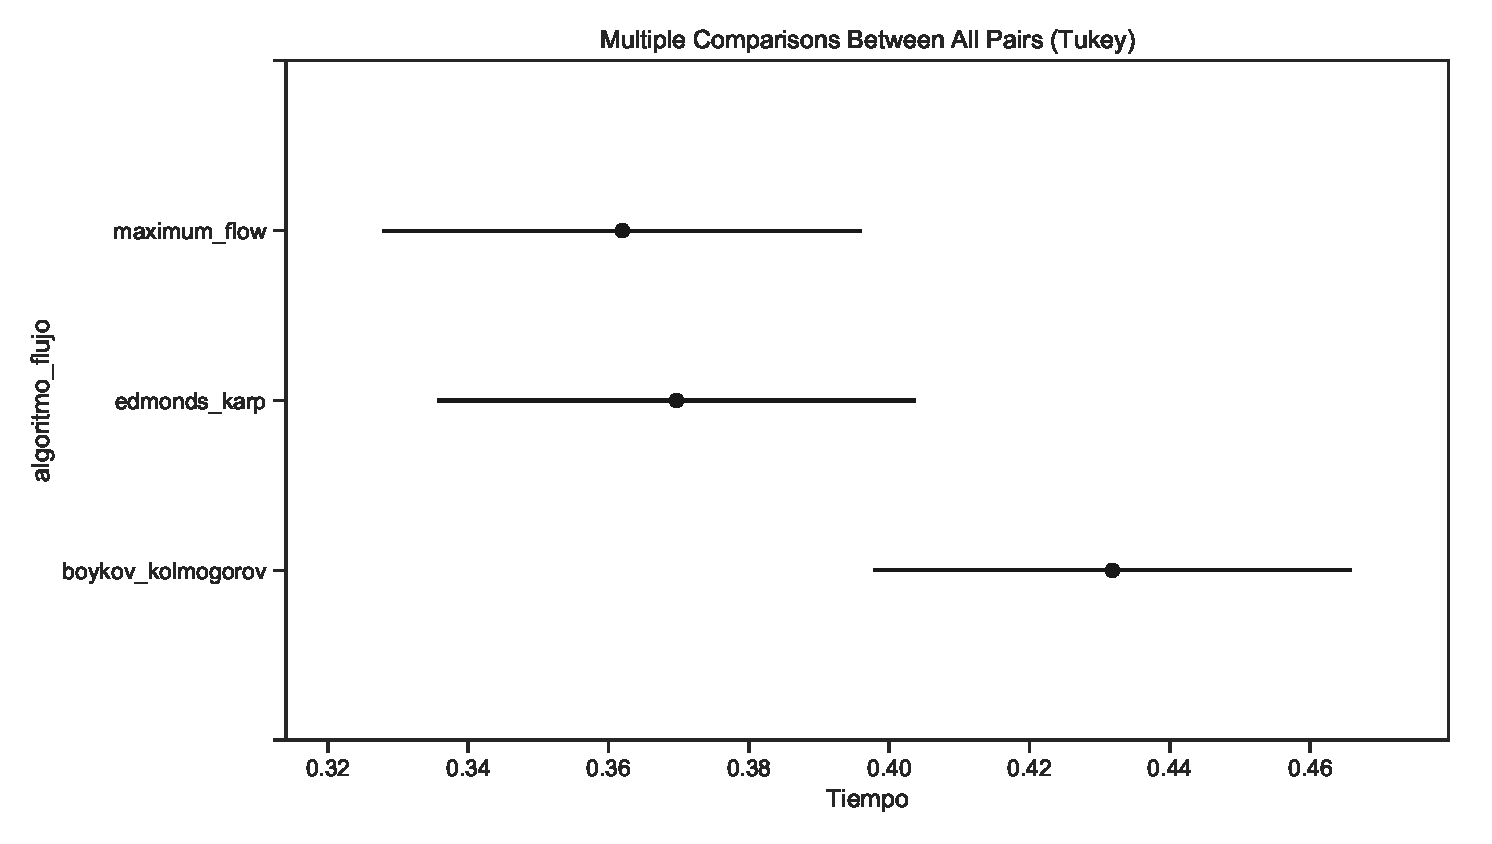
\includegraphics[scale=0.3, trim=0 0 0 20, clip=true]{Imagenes/tablatukeyalgoritmoflujo.eps}}
\subfigure[\textit{Tukey}:Tiempo vs densidad del grafo]{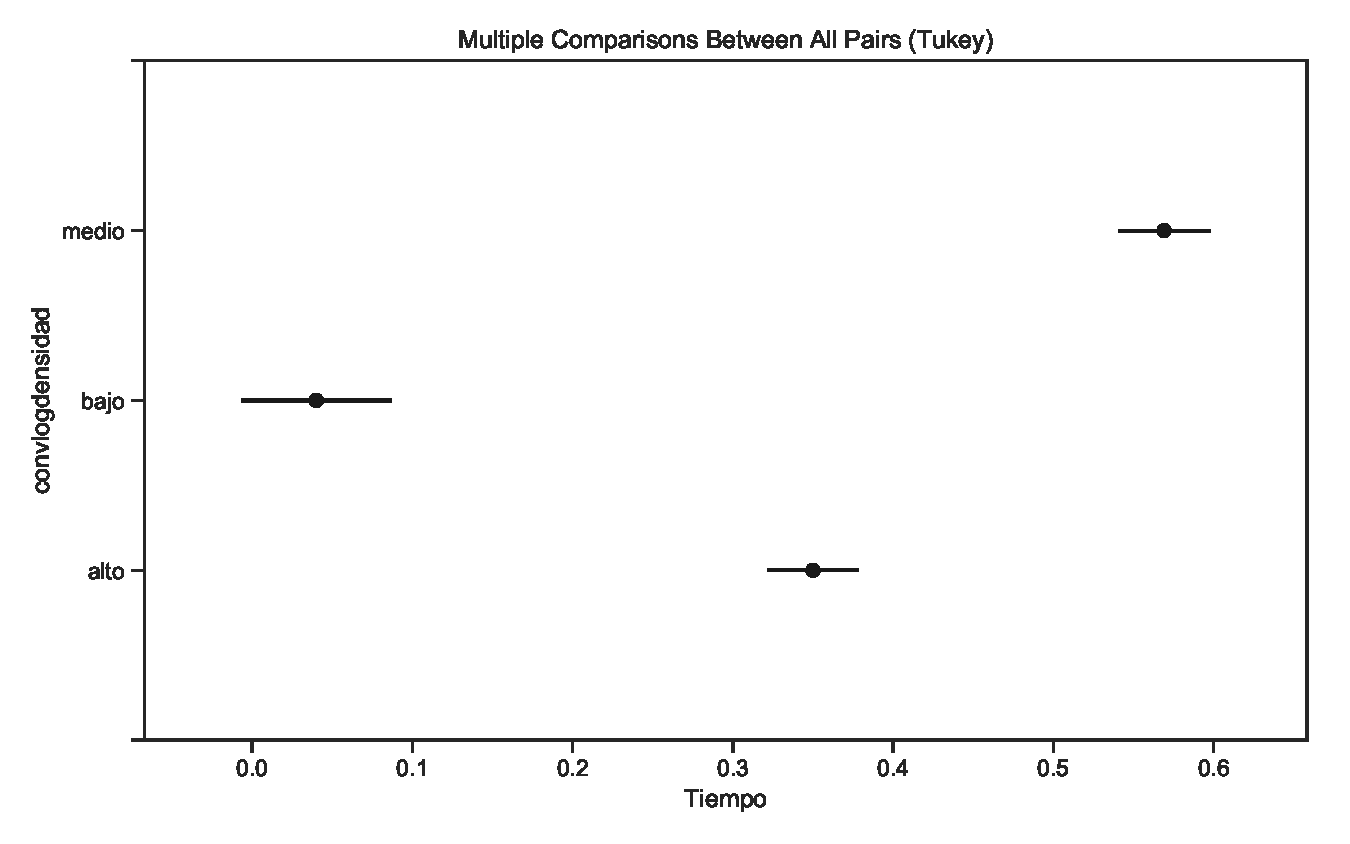
\includegraphics[scale=0.3, trim=0 0 0 20, clip=true]{Imagenes/tablatukeyconvlogdensidad.eps}}
\subfigure[\textit{Tukey}:Tiempo vs generador]{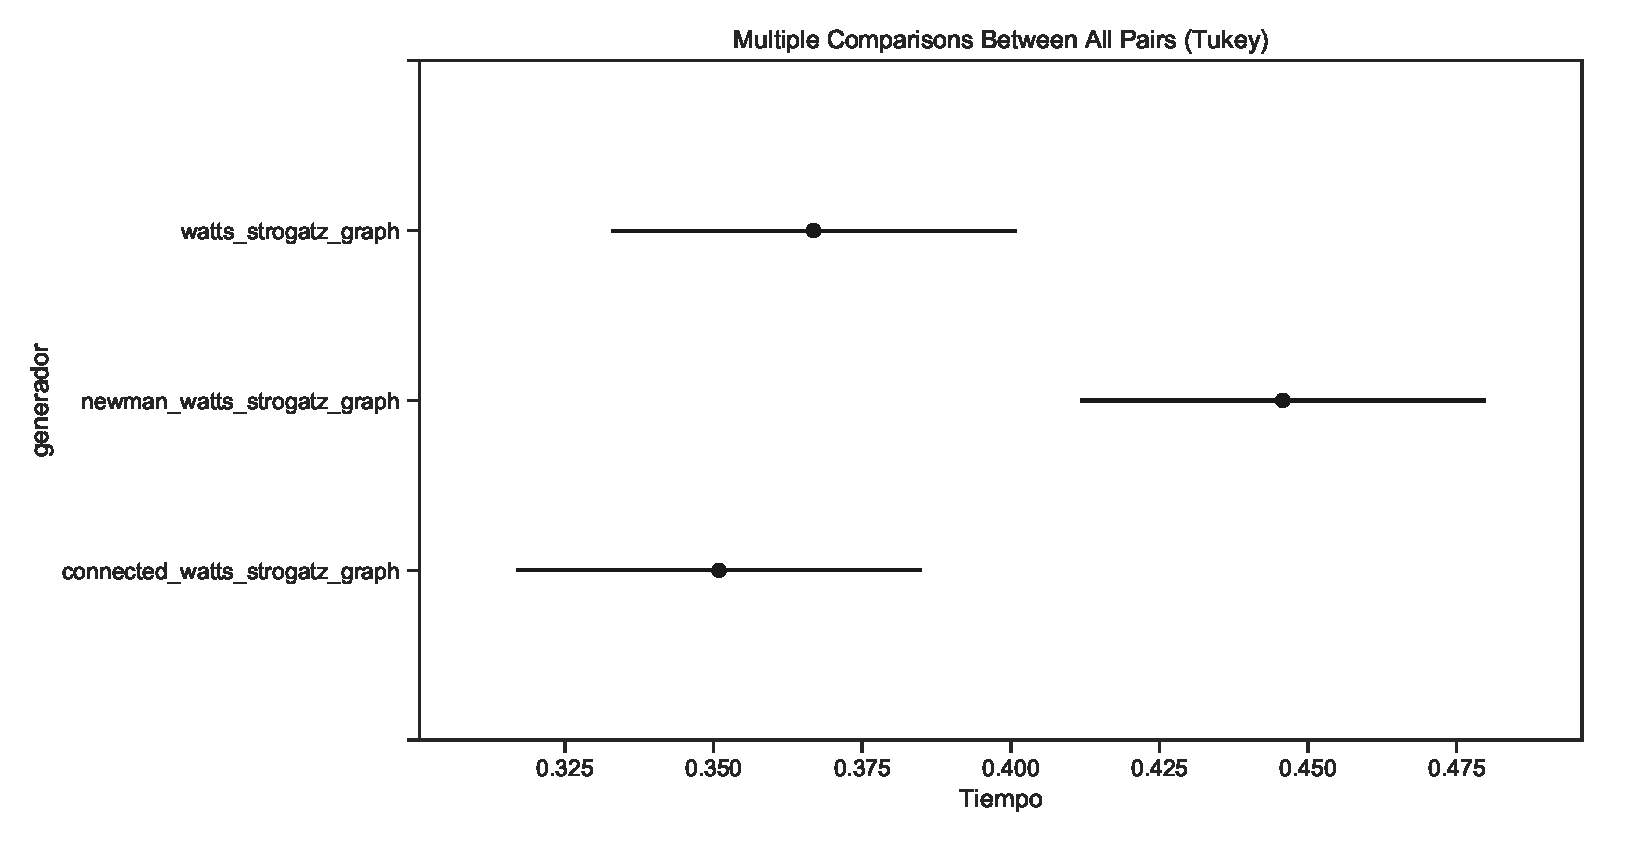
\includegraphics[scale=0.3,  trim=0 0 0 20, clip=true ]{Imagenes/tablatukeygenerador.eps}}
\subfigure[\textit{Tukey}:Tiempo vs vértices]{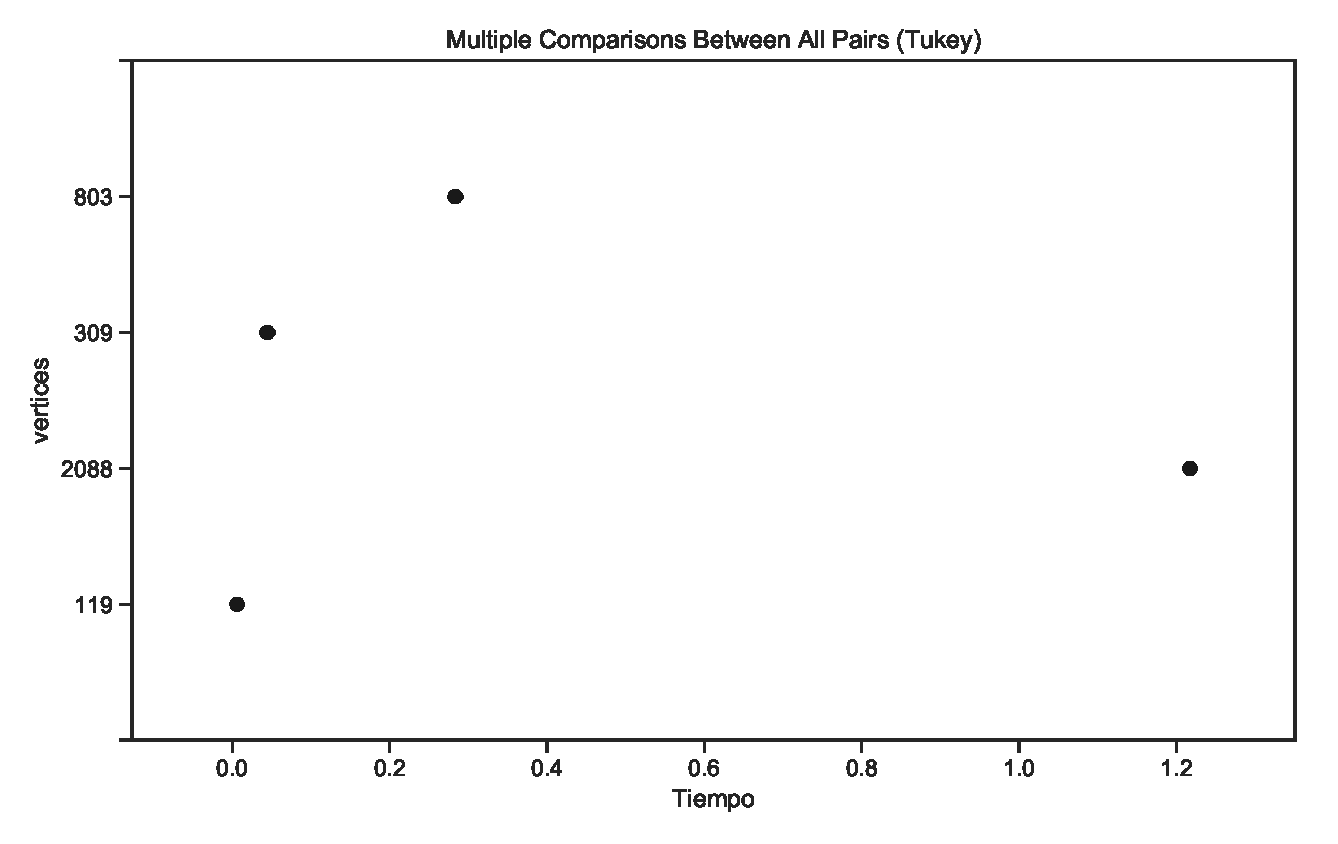
\includegraphics[scale=0.3,  trim=0 0 0 20, clip=true ]{Imagenes/tablatukeyvertices.eps}}

\caption{Intervalos de confianza de \textit{Tukey}}
\label{fig:Fig3}
\end{figure}

%\begin{figure}[htbp]
%
%\begin{subfigure}{0.5\textwidth}
%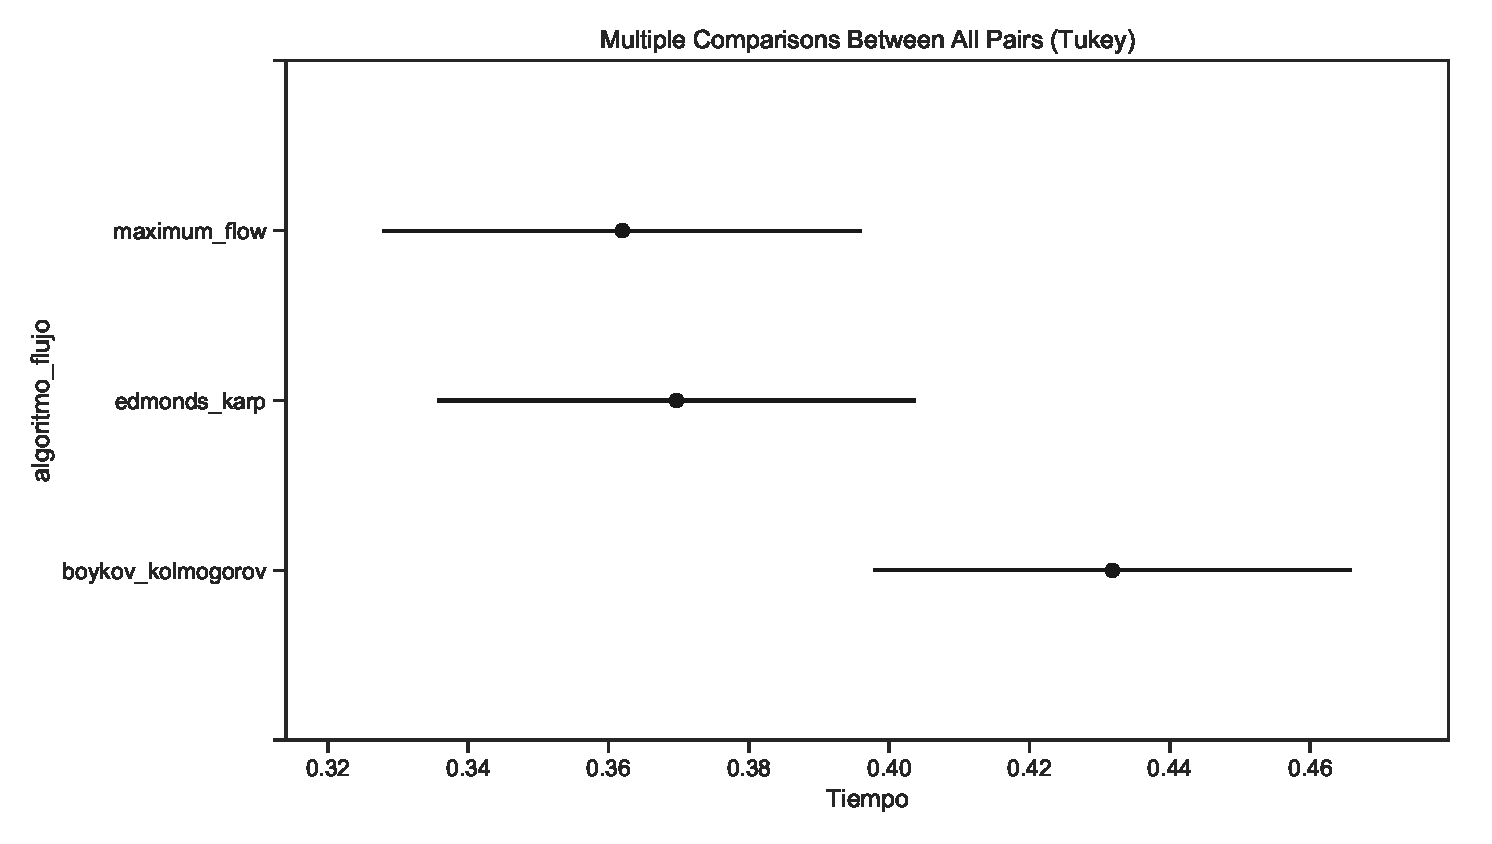
\includegraphics[scale=0.6, width=\textwidth, trim=0 0 0 20, clip=true]{Imagenes/tablatukeyalgoritmoflujo.eps} 
%\caption{}
%%\label{fig:AUSG_shellUnc}
%\end{subfigure}

%\begin{subfigure}{0.5\textwidth}
%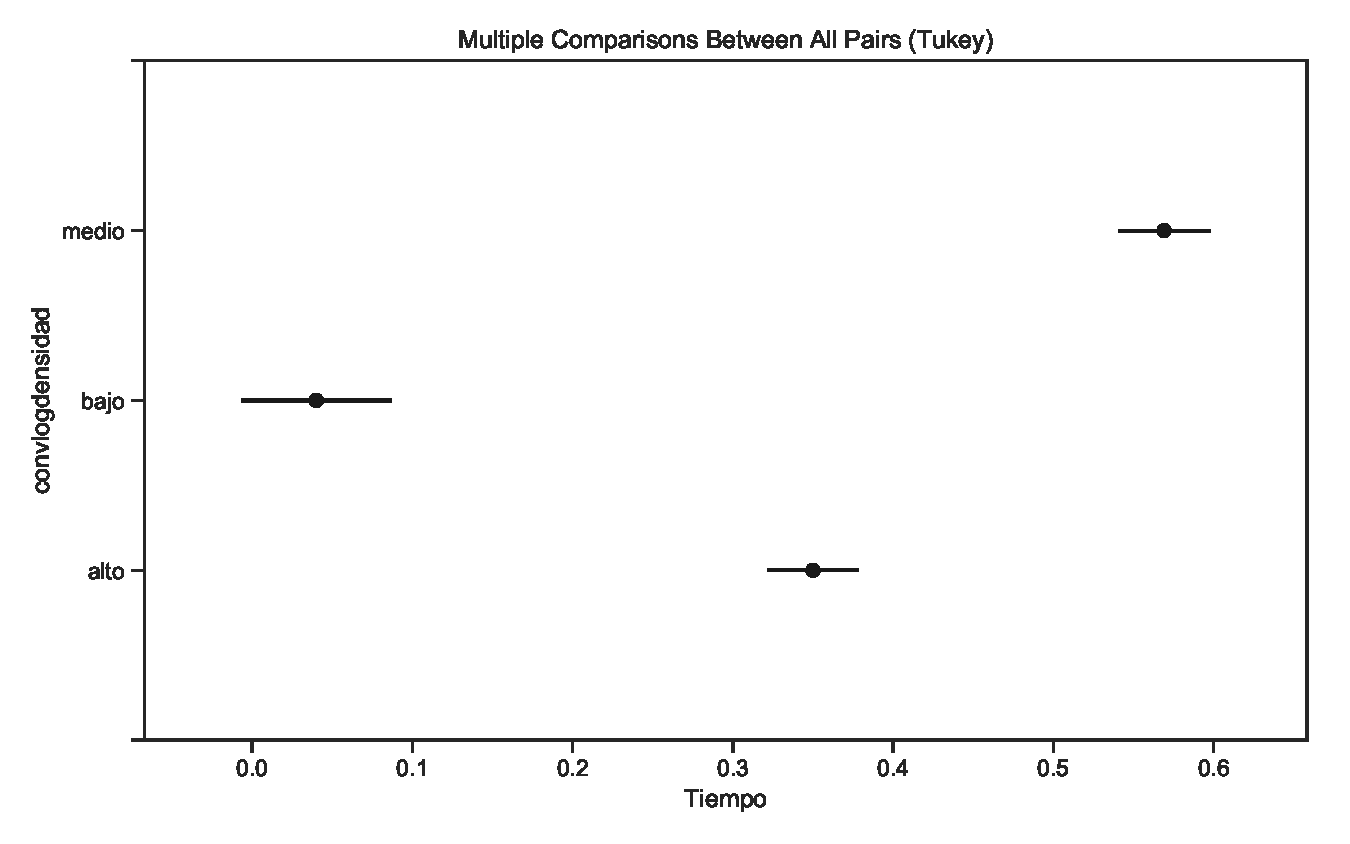
\includegraphics[scale=0.6, width=\textwidth, trim=0 0 0 20, clip=true]{Imagenes/tablatukeyconvlogdensidad.eps}
%\caption{\textit{Tukey}:Tiempo vs densidad del grafo}
%%\label{fig:AUSG_shellUncW}
%\end{subfigure}
%
%\begin{subfigure}{0.5\textwidth}
%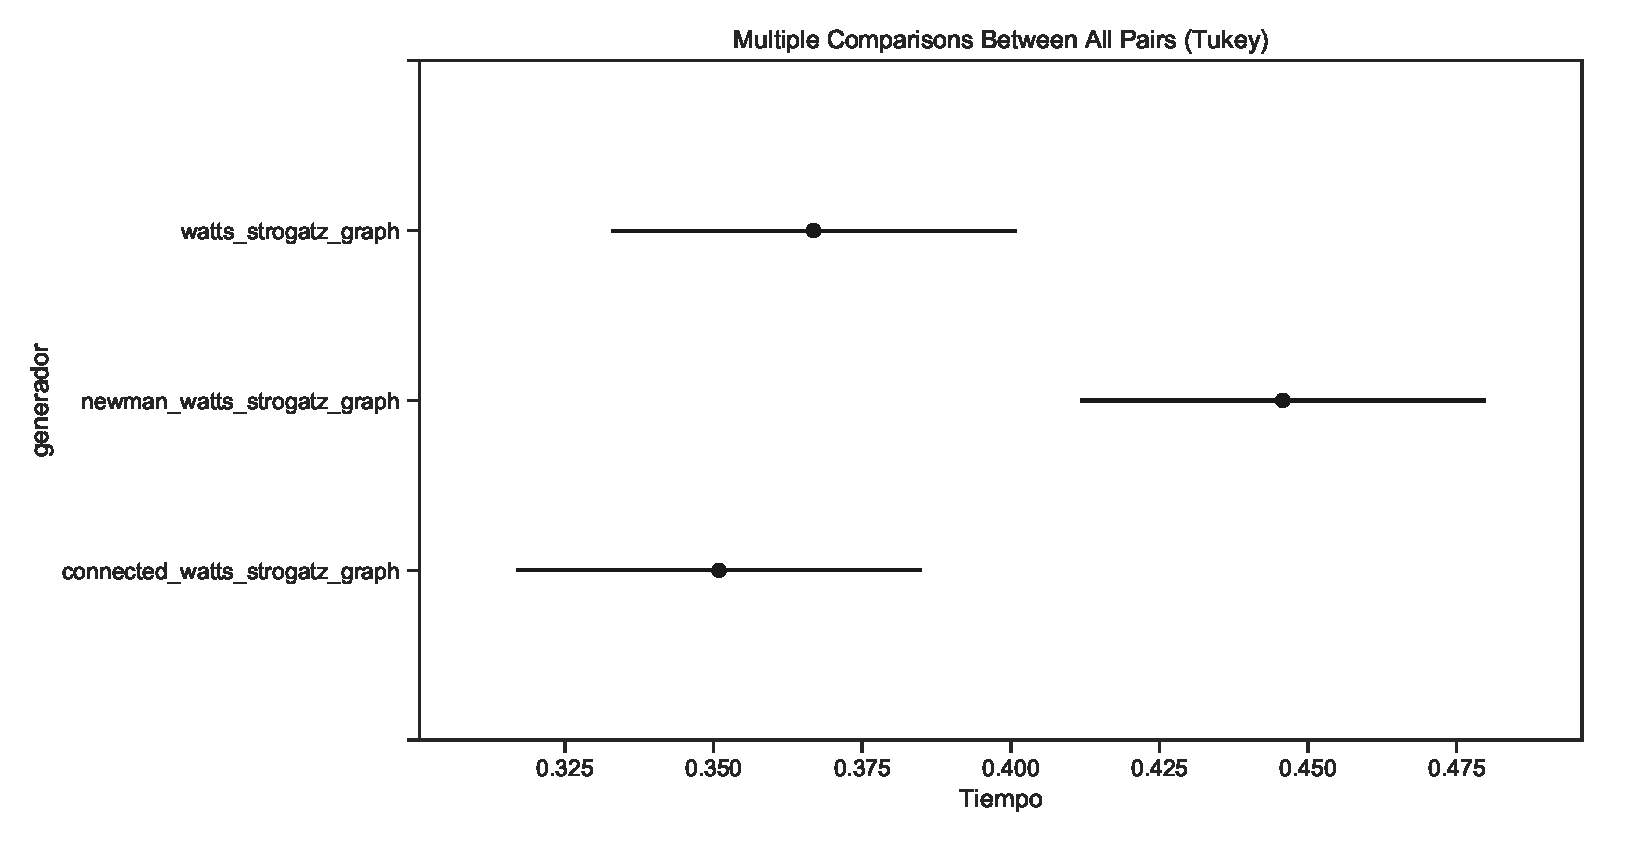
\includegraphics[scale=0.6, width=\textwidth, trim=0 0 0 20, clip=true]{Imagenes/tablatukeygenerador.eps}
%\caption{\textit{Tukey}:Tiempo vs generador}
%%\label{fig:AUSG_shelldEx}
%\end{subfigure}
%
%\begin{subfigure}{0.5\textwidth}
%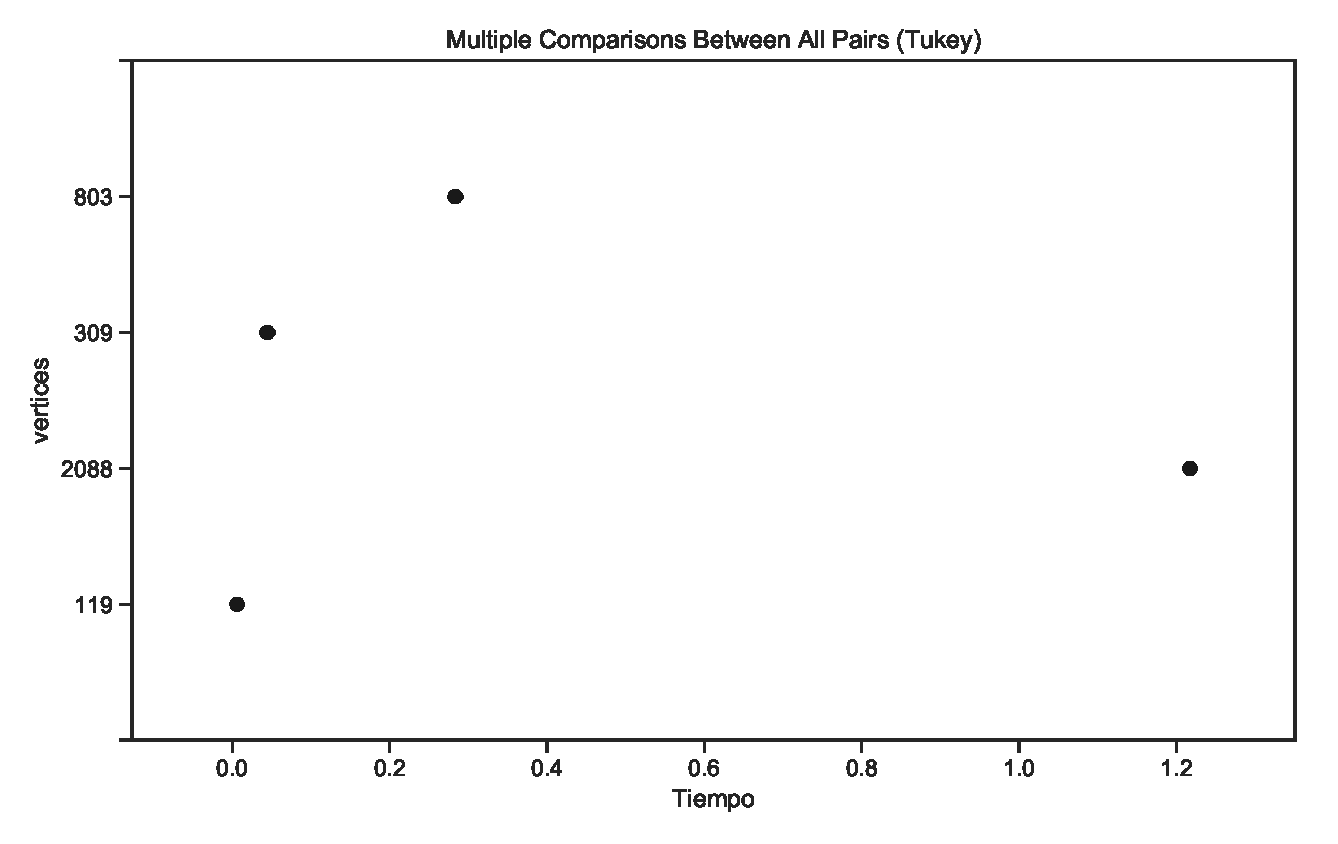
\includegraphics[scale=0.6, width=\textwidth, trim=0 0 0 20, clip=true]{Imagenes/tablatukeyvertices.eps}
%\caption{\textit{Tukey}:Tiempo vs vértices}
%%\label{fig:AUSG_shelldExW}
%\end{subfigure}
% 
%\caption{Intervalos de confianza de \textit{Tukey}}
%\label{fig:Fig3}
%\end{figure}

Del análisis del algoritmo de flujo se aprecia que se mantiene el algoritmo de \textit{Boykov Kolmogorov} 
como el de intervalo de desviación más amplio, y por tanto afecta más, en el par donde se combina. Para la densidad del grafo se aprecia que a pesar de existir diferencia en todos los pares, el que más influye es de la combinación medio con bajo niveles de densidad, se aprecia que el bajo tiene un intervalo mayor, pero el medio posee valores más altos, lo que significa que existe más diferencia entre los valores del rango bajo, pero los de nivel medio influyen más. Para el caso del generador de grafos, se aprecia similitud en los intervalos, por lo que más influye el \textit{Watts Strogatz Newman}. Según la cantidad de vértices en la prueba de \textit{Tukey} no existe diferencia significativa entre los límites superiores e inferiores, y se mantiene que más influye el de mayor cantidad de vértices.

Para conocer la relación entre todas las variables y su influencia en el tiempo de ejecución se realiza la interacción entre las ANOVAS de cada factor, los resultados muestran que los factores que más influyen en el tiempo de ejecución son el generador de grafos y el algoritmo seleccionado, en estos es donde el p\- valor es menor que 0,05 por tanto se rechaza la hipótesis nula, aceptando la hipótesis alternativa. Los resultados globales se muestran en el cuadro siguiente:



% Table generated by Excel2LaTeX from sheet 'multianova'
\begin{table}[htbp]
  \centering
  \caption{Interacción entre ANOVAS de un factor vs tiempo de ejecución}
    \begin{tabular}{lrrrr}
    \toprule
          & \multicolumn{1}{c}{\textbf{sum\_sq}} & \multicolumn{1}{c}{\textbf{df}} & \multicolumn{1}{c}{\textbf{F}} & \multicolumn{1}{c}{\textbf{PR(>F)}} \\
    \midrule
    generador & 0.498 & 2     & 33.242 & 0.000\\
    algoritmo\_flujo & 1.7604 & 2     & 117.378 & 0.000 \\
    vertices & 0.000 & 3     & 0.000 & 1.000 \\
    convlogdensidad & 0.000 & 2     & 0.000 & 1.000 \\
    generador:algoritmo\_flujo & 0.008 & 4     & 0.278 & 0.891 \\
    algoritmo\_flujo:vertices & 2.603 & 6     & 57.877 & 0.000 \\
    vertices:convlogdensidad & 19.356 & 6     & 430.247 & 0.000 \\
    generador:vertices & 48.5969 & 6     & 1080.187 & 0.000 \\
    generador:convlogdensidad & 0.471 & 4     & 15.719 & 0.000 \\
    Residual & 13.309 & 1775  &       &  \\
    \bottomrule
    \end{tabular}%
  \label{tab:addlabel}%
\end{table}%

El código que se empleó para realizar el análisis estadístico es el siguiente:

\newpage
\lstinputlisting[language=Python, firstline=7, lastline=19]{Tarea4Estadisticsfinal.py}
\lstinputlisting[language=Python, firstline=24, lastline=45]{Tarea4Estadisticsfinal.py}
\lstinputlisting[language=Python, firstline=73, lastline=108]{Tarea4Estadisticsfinal.py}

%\begin{figure}[h]
%    \centering
%    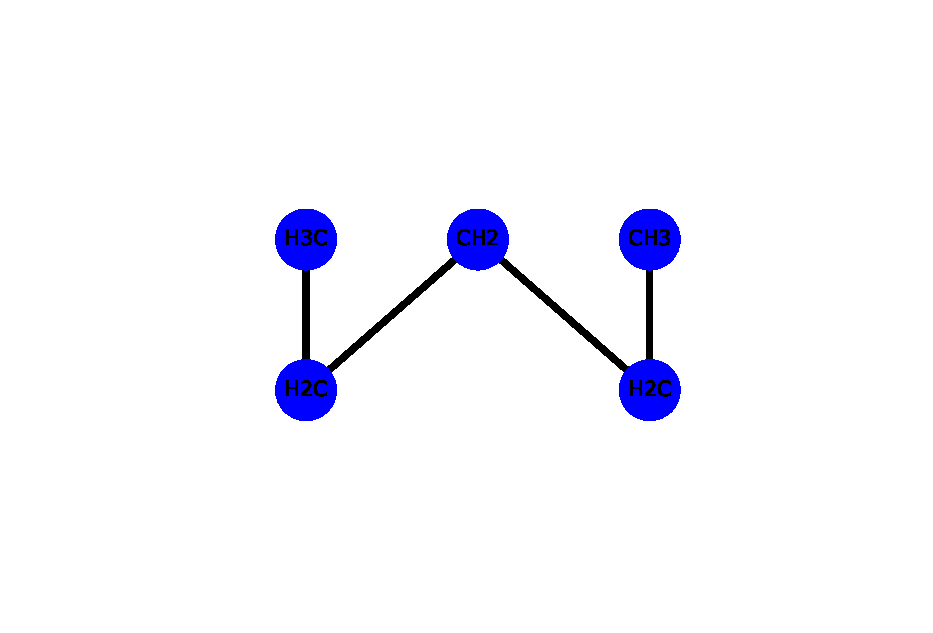
\includegraphics[scale=0.6]{Imagenes/Fig01.eps}
%    \caption{Histogramas de Algoritmos (cant valores vs media): azul-BC, rojo-MC, verde-GC, amarillo-MF y rosado-MS}
%    \label{fig:Fig01}
%\end{figure}
\newpage


\bibliography{Referencias_4}
\bibliographystyle{plainnat}
\end{document}
